\documentclass[a4paper,10pt,twoside]{article}

\usepackage[top=1in, bottom=1in, left=1in, right=1in]{geometry}
\usepackage[utf8]{inputenc}
\usepackage[spanish,es-ucroman,es-noquoting]{babel}
\usepackage{setspace}
\usepackage{fancyhdr}
\usepackage{lastpage}
\usepackage{amsmath}
\usepackage{amsfonts}
\usepackage{verbatim}
\usepackage{graphicx}
\usepackage{float}
\usepackage{algorithmic}
\usepackage{tikz}
\usepackage{ gensymb }
\usetikzlibrary{calc}
\usetikzlibrary{decorations.pathreplacing}


% Evita que el documento se estire verticalmente para ocupar
% el espacio vacío en cada página.
\raggedbottom


%%%%%%%%%% Configuración de Fancyhdr - Inicio %%%%%%%%%%
\pagestyle{fancy}
\thispagestyle{fancy}
\lhead{RTP2, Organización del Computador II}
\renewcommand{\footrulewidth}{0.4pt}
\cfoot{\thepage /\pageref{LastPage}}

\fancypagestyle{caratula} {
   \fancyhf{}
   \cfoot{\thepage /\pageref{LastPage}}
   \renewcommand{\headrulewidth}{0pt}
   \renewcommand{\footrulewidth}{0pt}
}
%%%%%%%%%% Configuración de Fancyhdr - Fin %%%%%%%%%%


%%%%%%%%%% Configuración de Algorithmic - Inicio %%%%%%%%%%
% Entorno propio para customizar la presentación del pseudocódigo
\newenvironment{pseudocodigo}
    {\vspace{0.5em} \begin{algorithmic}}
    {\end{algorithmic} \vspace{0.5em}}

% Alinear comentarios a la derecha
\renewcommand{\algorithmiccomment}[1]{\hfill \{#1\}}
%%%%%%%%%% Configuración de Algorithmic - Fin %%%%%%%%%%


%%%%%%%%%% Macros de tikz - Inicio %%%%%%%%%%
% Uso: \registroCuatro{etiqueta}{x}{y}{a4}{a3}{a2}{a1}
\newcommand{\registroCuatro}[7]{
    \ifthenelse{\equal{#1}{}}{}{
        \draw (#2, {#3 + 0.5}) node[anchor=east]{#1};
    }

    \draw   (#2, #3) rectangle +(4, 1) +(2, 0.5) node{#4}
          ++(4, 0)   rectangle +(4, 1) +(2, 0.5) node{#5}
          ++(4, 0)   rectangle +(4, 1) +(2, 0.5) node{#6}
          ++(4, 0)   rectangle +(4, 1) +(2, 0.5) node{#7};          
}

% Uso: \registroOcho{etiqueta}{x}{y}{a8}{a7}{a6}...{a1}
\newcommand{\registroOcho}[9]{
    \def\etiqueta{#1}
    \def\x{#2}
    \def\y{#3}
    \def\aviii{#4}
    \def\avii{#5}
    \def\avi{#6}
    \def\av{#7}
    \def\aiv{#8}
    \def\aiii{#9}
    \registroOchoX    
}
\newcommand{\registroOchoX}[2]{ % Auxiliar - no usar directamente
    \def\aii{#1}
    \def\ai{#2}
    \ifthenelse{\equal{\etiqueta}{}}{}{
        \draw (\x, {\y + 0.5}) node[anchor=east]{\etiqueta};
    }
    \filldraw[fill=white]
        (\x, \y) rectangle +(2, 1) +(1, 0.5) node{\aviii}
        ++(2, 0) rectangle +(2, 1) +(1, 0.5) node{\avii}
        ++(2, 0) rectangle +(2, 1) +(1, 0.5) node{\avi}
        ++(2, 0) rectangle +(2, 1) +(1, 0.5) node{\av}
        ++(2, 0) rectangle +(2, 1) +(1, 0.5) node{\aiv}
        ++(2, 0) rectangle +(2, 1) +(1, 0.5) node{\aiii}
        ++(2, 0) rectangle +(2, 1) +(1, 0.5) node{\aii}
        ++(2, 0) rectangle +(2, 1) +(1, 0.5) node{\ai};
}


% Uso: \registroDieciseis{etiqueta}{x}{y}{a16}{a15}{a14}...{a1}
\newcommand{\registroDieciseis}[9]{
    \def\etiqueta{#1}
    \def\x{#2}
    \def\y{#3}
    \def\axvi{#4}
    \def\axv{#5}
    \def\axiv{#6}
    \def\axiii{#7}
    \def\axii{#8}
    \def\axi{#9}
    \registroDieciseisX
}
\newcommand{\registroDieciseisX}[9]{ % Auxiliar - no usar directamente
    \def\ax{#1}
    \def\aix{#2}
    \def\aviii{#3}
    \def\avii{#4}
    \def\avi{#5}
    \def\av{#6}
    \def\aiv{#7}
    \def\aiii{#8}
    \def\aii{#9}
    \registroDieciseisXX
}
\newcommand{\registroDieciseisXX}[1]{ % Auxiliar - no usar directamente
    \def\ai{#1}
    \ifthenelse{\equal{\etiqueta}{}}{}{
        \draw (\x, {\y + 0.5}) node[anchor=east]{\etiqueta};
    }
    \filldraw[fill=white]
        (\x, \y) rectangle +(1, 1) +(0.5, 0.5) node{\axvi}
        ++(1, 0) rectangle +(1, 1) +(0.5, 0.5) node{\axv}
        ++(1, 0) rectangle +(1, 1) +(0.5, 0.5) node{\axiv}
        ++(1, 0) rectangle +(1, 1) +(0.5, 0.5) node{\axiii}
        ++(1, 0) rectangle +(1, 1) +(0.5, 0.5) node{\axii}
        ++(1, 0) rectangle +(1, 1) +(0.5, 0.5) node{\axi}
        ++(1, 0) rectangle +(1, 1) +(0.5, 0.5) node{\ax}
        ++(1, 0) rectangle +(1, 1) +(0.5, 0.5) node{\aix}
        ++(1, 0) rectangle +(1, 1) +(0.5, 0.5) node{\aviii}
        ++(1, 0) rectangle +(1, 1) +(0.5, 0.5) node{\avii}
        ++(1, 0) rectangle +(1, 1) +(0.5, 0.5) node{\avi}
        ++(1, 0) rectangle +(1, 1) +(0.5, 0.5) node{\av}
        ++(1, 0) rectangle +(1, 1) +(0.5, 0.5) node{\aiv}
        ++(1, 0) rectangle +(1, 1) +(0.5, 0.5) node{\aiii}
        ++(1, 0) rectangle +(1, 1) +(0.5, 0.5) node{\aii}
        ++(1, 0) rectangle +(1, 1) +(0.5, 0.5) node{\ai};
}
%%%%%%%%%% Macros de tikz - Fin %%%%%%%%%%


%%%%%%%%%% Macros misceláneos - Inicio %%%%%%%%%%
\newcommand{\xmm}[1]{\texttt{XMM#1}}
\newcommand{\rax}{\texttt{RAX}}
\newcommand{\rbx}{\texttt{RBX}}
\newcommand{\rcx}{\texttt{RCX}}
\newcommand{\rdx}{\texttt{RDX}}
\newcommand{\rbp}{\texttt{RBP}}
\newcommand{\rsp}{\texttt{RSP}}
\newcommand{\reg}[1]{\texttt{R#1}}
\newcommand{\asm}[1]{\texttt{\uppercase{#1}}}
\newcommand{\INDSTATE}[1][1]{\STATE\hspace{#1\algorithmicindent}}
%%%%%%%%%% Macros misceláneos - Fin %%%%%%%%%%


\begin{document}


%%%%%%%%%%%%%%%%%%%%%%%%%%%%%%%%%%%%%%%%%%%%%%%%%%%%%%%%%%%%%%%%%%%%%%%%%%%%%%%
%% Carátula                                                                  %%
%%%%%%%%%%%%%%%%%%%%%%%%%%%%%%%%%%%%%%%%%%%%%%%%%%%%%%%%%%%%%%%%%%%%%%%%%%%%%%%


\thispagestyle{caratula}

\begin{center}


\includegraphics[height=2cm]{DC.png} 
\hfill

\includegraphics[height=2cm]{UBA.jpg} 

\vspace{2cm}

Departamento de Computación,\\
Facultad de Ciencias Exactas y Naturales,\\
Universidad de Buenos Aires

\vspace{4cm}

\begin{Huge}
RTP2
\end{Huge}

\vspace{0.5cm}

\begin{Large}
Organización del Computador II
\end{Large}

\vspace{1cm}

Segundo Cuatrimestre de 2013

\vspace{4cm}

Grupo: \textbf{Frambuesa a la Crema}

\vspace{0.5cm}

\begin{tabular}{|c|c|c|}
\hline
Apellido y Nombre & LU & E-mail\\
\hline
B\'alsamo, Facundo		& 874/10 & facundobalsamo@gmail.com\\
Lasso, Nicol\'as 			& 763/10 & lasso.nico@gmail.com\\
Rodr\'iguez, Agust\'in	& 120/10 & agustinrodriguez90@hotmail.com\\
\hline
\end{tabular}

\end{center}

\newpage


%%%%%%%%%%%%%%%%%%%%%%%%%%%%%%%%%%%%%%%%%%%%%%%%%%%%%%%%%%%%%%%%%%%%%%%%%%%%%%%
%% Índice                                                                    %%
%%%%%%%%%%%%%%%%%%%%%%%%%%%%%%%%%%%%%%%%%%%%%%%%%%%%%%%%%%%%%%%%%%%%%%%%%%%%%%%


\tableofcontents

\newpage


%%%%%%%%%%%%%%%%%%%%%%%%%%%%%%%%%%%%%%%%%%%%%%%%%%%%%%%%%%%%%%%%%%%%%%%%%%%%%%%
%% Introducción                                                              %%
%%%%%%%%%%%%%%%%%%%%%%%%%%%%%%%%%%%%%%%%%%%%%%%%%%%%%%%%%%%%%%%%%%%%%%%%%%%%%%%


\section{Introducción}

El lenguaje C es uno de los más eficientes en cuestión de performance, pero esto no quiere decir que sea óptimo para todos los casos o que no haya campos en los que pueda utilizarse una opción mejor.
Para comprobar esto, experimentamos con el set de instrucciones SIMD de la arquitectura Intel. Vamos a procesar imágenes mediante la aplicación de ciertos filtros y estudiaremos la posible ventaja que puede tener un código en Assembler con respecto a uno en C.
Implementaremos los filtros en ambos lenguajes para luego poder comparar la performance de cada uno y evaluar las ventajas y/o desventajas de cada uno.



%%%%%%%%%%%%%%%%%%%%%%%%%%%%%%%%%%%%%%%%%%%%%%%%%%%%%%%%%%%%%%%%%%%%%%%%%%%%%%%
%% Desarrollo                                                                %%
%%%%%%%%%%%%%%%%%%%%%%%%%%%%%%%%%%%%%%%%%%%%%%%%%%%%%%%%%%%%%%%%%%%%%%%%%%%%%%%


\section{Desarrollo y Resultados}

\subsection{Filtro Color}

Este filtro consiste b\'asicamente en dados un color y una distancia pasados como par\'ametros, procesa cada pixel de una im\'agen a color evaluando si el color del mismo se ''aleja'' m\'as de la distancia del par\'ametro, y si eso pasa, el p\'ixel se transforma a escala de grises, sino lo mantiene igual. Esto logra el efecto de resaltar un color en una im\'agen.

\subsubsection{Implementación en C}
Mediante dos ciclos anidados, se recorre la im\'agen por cada componente de color de cada pixel. Por cada pixel se levantan sus 3 colores RGB para calcular la distancia a los 3 colores RGB pasados por par\'ametro. Si el color de la im\'agen supera esa distancia, entonces en el p\'ixel que se est\'a procesando quedan sus 3 colores iguales unos con otros, logrando convertirse a blanco y negro. Si el color no supera la distancia, debe mantenerse tal cual, logrando as\'i ser resaltado.\\
Se define la distancia entre colores c\'omo:\\

\begin{center}
$distancia((r, g, b), (rc, gc, bc)) = \sqrt{(r - rc)^2 + (g - gc)^2 + (b - bc)^2}$
\end{center}

Para pasar a blanco y negro el p\'ixel, ponemos en cada canal de color (rgb), el mismo valor: $\frac{r + g + b}{3}$.

\subsubsection{Implementación en Assembler}
Haciendo uso de los registros \emph{XMM} por cada acceso a memoria se pueden traer 16 bytes con lo cual la cantidad de accesos a memoria decrementa 
considerablemente, haciendo que en comparaci\'on con el co\'odigo en C este sea mas optimo ya que el acceso a memoria es de las operaciones que mas 
consumen en cantidad de ciclos haciendo que disminuya la performance. Esto podr\'a apreciarse en la secc\'on de resultados.\newline
Al levantar los 16 bytes, lo primero que realizo es copiar estos 16 bytes en otros 2 registros \emph{XMM} para luego ordernarlos mediante la instrucc\'on
de Shuffle para que queden de la siguiente forma:

\begin{center}
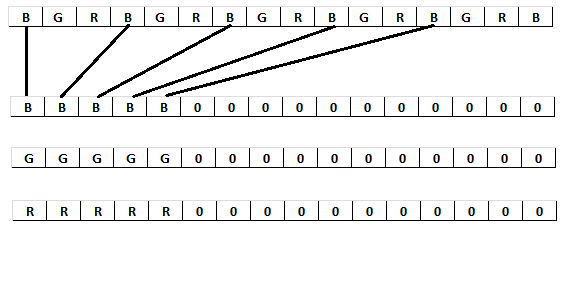
\includegraphics{imagenes/ImagenReorden.png}  
\end{center}

Luego le restamos a cada uno de los datos dentro de nuestros registros, un valor rc, bc o gc que es pasado por par\'matro, seg\'un se explica al
comienzo de esta secci\'on. Una considera\'on que vale la pena aclarar es que la resta es una diferencia absoluta. Este recaudo se tuvo que tomar dado 
que los bytes de la matriz son \emph{unsigned char} con lo cual si restabamos a un valor mas chico un valor mas grande esto pod\'ia confundirse y dejarnos
un valor que de ser una resta con sino ser\'ia v\'alido pero para nosotros no era util. Siendo esto, se toma compara el valor m\'as grande de cada dato
dentro del registro y el mas chico y se separan ambos en dos registros distintos. Luego se hace una resta del modo MAX - MIN dejando la resta sin signo
como quer\'iamos. A modo de ejemplo dejamos la siguiente imagen:

\begin{center}
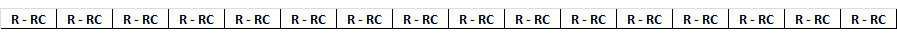
\includegraphics[width=16cm]{imagenes/resta.png} 
\end{center}

Una vez hecha la resta, se procede a convertir a float ya que las siguientes operaciones son multiplicaci\'on, suma y raiz cuadrada para la cual necesitamos
convertir nuestros datos a Float. La cuenta realizada por cada pixel es la siguiente:

\begin{center}
 $\sqrt{(r - rc)^2 + (g - gc)^2 + (b - bc)^2}$
\end{center}

Al final de toda la operaci\'on dejamos en 2 registros los 5 floats con cada una de estas operaciones en cada pixel. La siguiente imagen queda a forma de
entendimiento:

\begin{center}
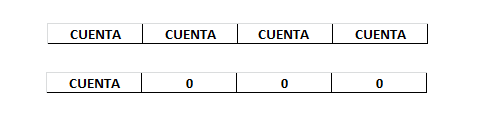
\includegraphics{imagenes/FinOperacion.png} 
\end{center}
 Un vez qu tenemos estos valores y luego de convertirlos a INT de tamaño Double word. Mediante el uso de la instrucci\'on PCMPGTD, comparamos que datos son
mayores y cuales son menores o iguales al valor pasado por parametro \emph{threshold} generando una mascara con valores 0xffffffff si el resultado de la 
operaci\'on dio \emph{true} y 0x0 en otro caso.\newline
Ya con esta m\'ascara generada, copiamos en 2 registros los valores originales de la matriz, y dejamos en uno los valores que queremos procesar usando la
instrucci\'on PAND y en otro los valores que queremos dejar como est\'an en el original usando PXOR de la m\'ascara y un PAND contra el registro. De esta
 manera negamos la m\'ascara y nos quedamos con los otros.\newline
Para terminar, procesamos los datos que debemos realizar la siguiente cuenta en para cada pixel:

\begin{center}
 $\frac{b + g + r}{3}$
\end{center}

Por \'ultimo solo le agregamos los resultados de los bits procesados al registro que tiene los datos originales y lo guardamos en la matriz de destino.

\subsubsection{Consideraci\'ones seg\'un optimizaciones}
\begin{itemize}
 \item Usando la herramienta \emph{objdump} desensamblamos el archivo .o de c\'odigo del filtro de Color. Al observar este c\'odigo, lo primero que notamos es
 que el compilador no us\'o instrucci\'ones de SIMD a pesar de que el procesador tenga esa caracteristica. Esto se debe a que al escribir en lenguaje C
no se puede hacer uso de estas operaciones a menos que usemos una librer\'ia aparte que haga uso de estas como puede ser \emph{libSIMDx86}.\newline
En cuanto a como se manipulas las variables locales, Se respetan las convenciones de pushear registros como r15 - r12 y rbx. Pero en casi todo el c\'odigo
se hace uso de las variables por parametros y se usa mucho la pila moviendo el registro rbp para recorrerla.\newline
\item Existen algunas optimizaciones que se pueden realizar a la hora de compilar el c\'odigo en C. Estas son -O1, -O2 o -O3, las cuales, siendo agregadas
como flags a la hora de compilar, mi c\'odigo ensamblado queda mucho m\'as \'optimo. En particular el flag -O1 hace que el tamaño del c\'odigo ensamblado
sea mucho menor que el c\'odigo ensablado sin optimizaci\'on. En particular al mirar el objdump de c\'odigo con -O1 se pudo apreciar que el c\'odigo era
mucho menor en cantidad de lineas y que la cantidad de registros pusheados a la pila fue mayor.\newline
El flag -O2 hace todas las optimizaciones que pueda en el c\'odigo que no est\'en involucradas con optimizaciones de espacio-tiempo. Y por \'ultimo el flags
-O3 abre todas las opmitizaciones de -O2 mas algunas extras con el fin de hacer aun m\'as optimo el c\'odigo.\footnote{Para mas informaci\'on revisar el
http://gcc.gnu.org/onlinedocs/gcc/Optimize-Options.html}\newline
\item Haciendo uso de las optimizaciones mencionadas anteriormente, se realizaron experimentos de performance usando el c\'odigo en ASM, en C y en C 
compilado con optimizacion -O1, -O2 y -O3. El siguiente gr\'afico muestra como el c\'odigo en C optimizado y el ASM son casi id\'enticos.

\begin{center}
 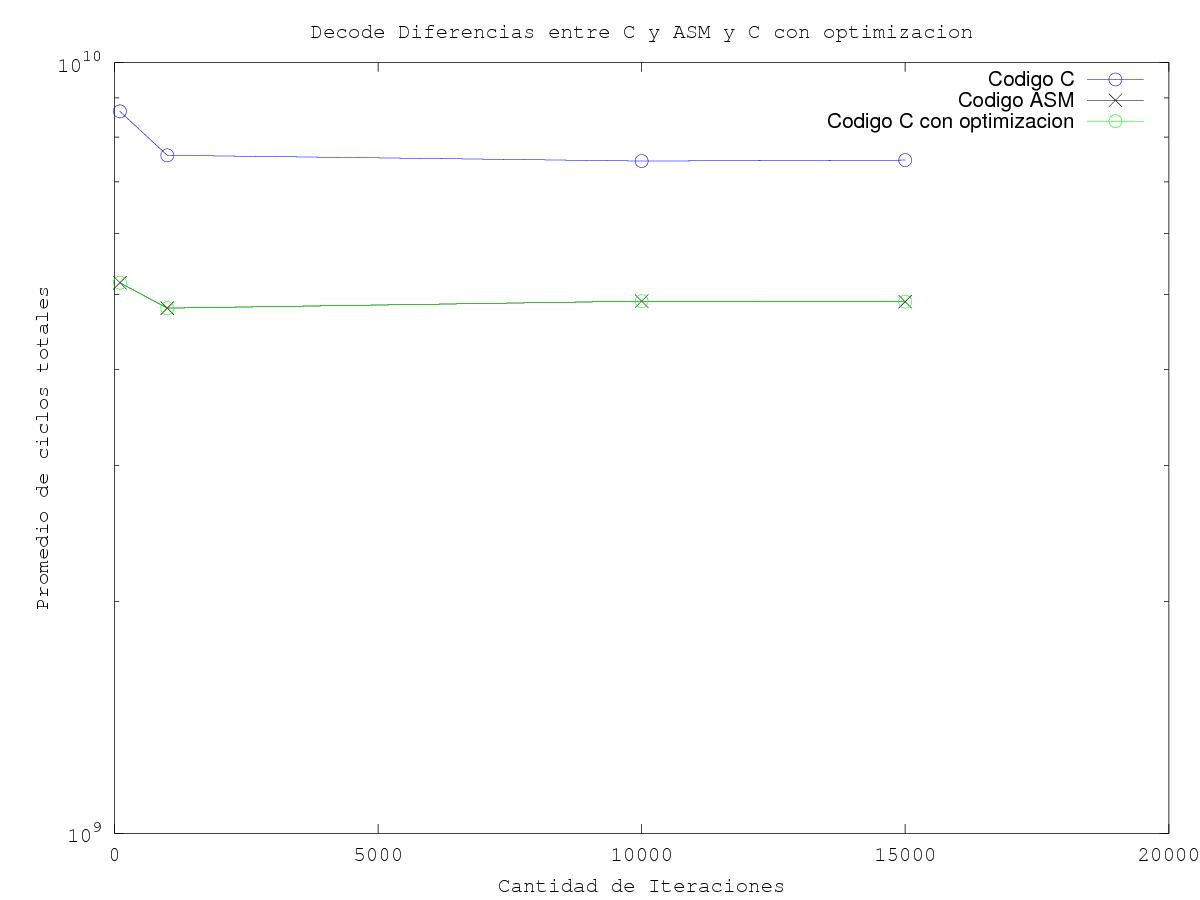
\includegraphics[scale=0.5]{imagenes/optimizacionC.jpg}
\end{center}

Esta medici\'on fue realizada cambiando la cantidad de iteraciones y midiendo cuantos ticks de procesador consume procesar el video completo. El 
problema de realizar las mediciones de esta manera es que el procesador switchea entre distintos procesos todo el tiempo haciendo que mi contador aumente
 al ejecutar procesos que no pertenecen a mi funci\'on y se cuenta en intervalos muy grandes provocando que la probabilidad de contar ticks de procesos
 exteriores sea mayor. Es por esta raz\'on que nuestra medici\'on no es lo suficientemente precisa. Una forma de hacerla mas precisa ser\'ia evaluando un
promedio de la cantidad de Ticks que consume por cada frame de cada iteraci\'on. Pero al trabajar en ordenes tan grandes deber\'iamos procesar demasiada
 informaci\'on que no viene al caso de lo que se queire mostrar.\newline

\end{itemize}

\subsubsection{Loop unrolling}
Loop unrolling, o desenrollado de ciclo en español, es una t\'ecnica de optimizaci\'on que consiste en transformar un bucle para mejorar la velocidad de ejecuci\'on de un programa. La transformaci\'on puede llevarse a cabo por el programador o por un compilador de optimizaci\'on.\\
La t\'ecnica se basa en eliminar las instrucciones que controlan el bucle, por ejemplo, reduciendo la cantidad de iteraciones que tiene que pasar un ciclo, evitando comparar menos veces si se termin\'o de iterar o no.\\
Por ejemplo:

\begin{center}
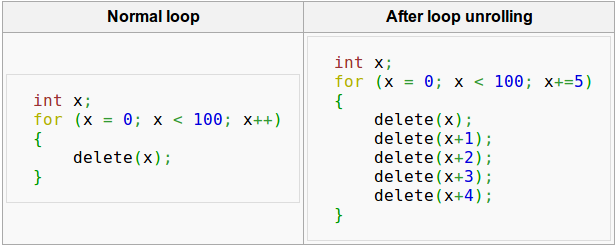
\includegraphics[scale=0.5]{imagenes/loopunrolling_ejemplo.png}
\end{center}

Como podemos ver, el ciclo desenrollado recorre menos veces, por lo tanto hace menos comparaciones. Pero corre con la gran desventaja de que se genera mucho m\'as c\'odigo.\\
Una forma de aplicarlo a nuestro filtro de color en C es procesar m\'as cantidad de p\'ixels. En nuestro filtro C com\'un procesamos de a 1 p\'ixel. Probamos procesar de a 2 p\'ixels, donde el procesamiento de columnas, o de ancho de la im\'agen se reduce a la mitad. Sin embargo, midiendo velocidades, no detectamos grandes diferencias, ya que esa optimizaci\'on no es muy significativa o el compilador de C tal vez haga esta optimizaci\'on.\\
Luego probamos optimizando m\'as, procesando de a 6 p\'ixels en el C y ahorrando ciertos accesos a memoria. Los resultados fueron m\'as notorios:

\begin{center}
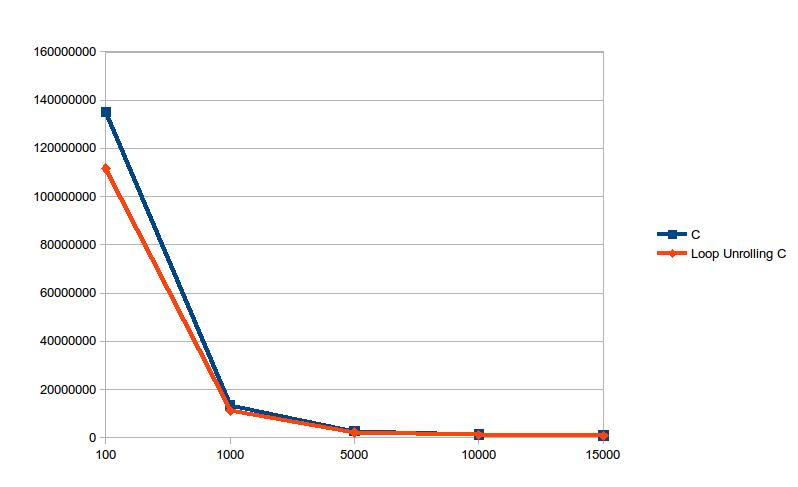
\includegraphics[scale=0.5]{imagenes/loopunrolling_c.jpg}
\end{center}

El eje x son la cantidad de iteraciones y el eje y es el tiempo que tard\'o para cierta cantidad de iteraciones.\\
En velocidad vemos la mejora del loop unrolling, pero en c\'odigo incrementa considerablemente.\\\\

En cuanto al c\'odigo ASM resulta m\'as complejo hacer esta optimizaci\'on ya que procesamos de a 5 p\'ixels, lo que entra en un registro XMM.\\
Lo que probamos fue copiar ese procesamiento de 5 p\'ixels, para procesar id\'enticamente la misma cantidad dentro del ciclo. Es decir que dentro de un mismo bucle procesamos 5 p\'ixels, y luego otros 5, procesando de a 10 en un mismo bucle. De esta manera nos ahorramos que se ejecuten las dos instrucciones de control del ciclo la mitad de las veces:\\

.ciclo:\\
CMP rcx, 0\\
JLE .fin\\

Midiendo tiempos de ejecuci\'on nos damos cuenta que no hay grandes diferencias con el ASM implementado sin aplicar esta t\'ecnica. Al parecer ahorrar 2 instrucciones b\'asicas de assembler para el tamaño de im\'agen que probamos (960 x 540), no es significativo.\\
Vale aclarar que la cantidad de pixels en ancho o en alto debe ser multiplo de 10, sino habr\'ia que tener ciertas consideraciones.

\subsubsection{Conversiones y extensiones de datos}
En varias secciones del c\'odigo en assembler de los filtros fue necesario extender o convertir los datos de entrada ya sea para realizar operaciones con
mayor precisi\'on o para poder operar con ellos.\newline

 Por ejemplo, en el filtro de color la extensi\'on y conversi\'on del dato fue necesaria a la hora de
 calcular la m\'ascara\footnote{Ver secci\'on 2.1.2}. La diferencia absoluta pudo calcularse sin ninguna operaci\'on extra pero cuando tuvimos que 
Multiplicar y sumar datos era posible que se superara el n\'umero 255, que es el mayor n\'umero representable con 8 bits. Por esta raz\'on se extendieron
los char de entrada en DoubleWords. Podr\'ia haber bastado con extender a Word pero luego necesitamos hacer una operaci\'on de raiz cuadrada con lo cual fue
m\'as \'optimo extender a DoubleWord y luego convertir a Float ya que de esta manera no perdemos precisi\'on en el \'ultimo c\'alculo. A continuaci\'on, 
result\'o necesario convertir de nuevo a dato Int Double Word. Para esto se us\'o la instrucci\'on CVTTPS2DQ ya que tiene la particularidad de truncar el 
n\'umero en lugar de redondear al m\'as cercano como hacen otras instrucciones por default y est\'a seteado en el flag 13 y 14 del registro MXCSR\footnote{Ver Manual de Intel volumen 1, secci\'on 10.2.3}.
 Vale aclararlo ya que a la hora de buscar diferencias entre filtros esto produjo una reducci\'on muy grande de diferencias. Por \'ultimo en la m\'ascara se comprimi\'o el dato 
de DoubleWord a Byte. Para la operaci\'on real con los datos que son guardados en la salida tambi\'en fue necesario realizar estas operaciones, se extendi\'o a 
Int de 32 bits y luego se convirti\'o a Float todo de una vez para que resulte m\'as \'optimo en lugar de primero desempaquetar a Word y luego a DoubleWord. Luego se
procedi\'o con las operaciones de suma y divisi\'on y se empaquet\'o de nuevo a Byte para insertarlo en la posici\'on de salida.



\subsection{Filtro Miniature}

Este filtro consiste en procesar una im\'agen para lograr un efecto miniatura. Consiste en que los objetos se vean pequeños o como de juguetes. Para esto se ''desenfoca'' la parte superior y la inferior de la im\'agen, quedando as\'i s\'olo el foco en la parte del medio, logrando tal efecto.



\subsubsection{Implementación en C}
Para esta implementaci\'on procesamos la imagen por bandas.
Para eso calculamos el límite de las bandas seg\'un los par\'ametros de entrada. Luego recorremos mediante dos ciclos la banda del medio y la dejamos igual, no hacemos ninguna transformaci\'on.\\
Luego dentro de un ciclo que cuenta las iteraciones, hacemos el procesamiento de ''desenfoque'' de la banda superior primero y luego la inferior.\\
Para desenfocar una banda, se recorre mediante dos ciclos que me permiten levantar cada color de cada pixel. Teniendo un componente de color de un pixel, se calcula el nuevo valor que debe tener el mismo. Para este c\'alculo se procesa la subimagen que hay alrededor del píxel, haciendo el c\'alculo por color, la multiplicamos por la matriz M, y vamos acumulando ese producto.\\
Para evitar la saturaci\'on, al resultado lo dividimos por 6, que es la suma de las componentes de la matriz M. Con el nuevo valor obtenido, lo pasamos a la im\'agen resultante. Seguimos procesando hasta finalizar la banda.
Para incrementar el efecto, lo que hacemos es, por iteraci\'on, guardar el p\'ixel desenfocado, para que en la siguiente iteración lo procese otra vez.\\

$M = \begin{pmatrix}
  0.01 & 0.05 & 0.18 & 0.05 & 0.01 \\
  0.05 & 0.32 & 0.64 & 0.32 & 0.05 \\
  0.18 & 0.64 & 1 & 0.64 & 0.18 \\
  0.05 & 0.32 & 0.64 & 0.32 & 0.05 \\
  0.01 & 0.05 & 0.18 & 0.05 & 0.01 \\
 \end{pmatrix}$

\subsubsection{Implementación en Assembler}
Para la implementaci\'on en assembler de este filtro, la diferencia mas sifnificativa contra la implementaci\'on en C, fue la forma de levantar los registros.
Usando los registros \emph{XMM} se levantaron 5 registros de 16 bytes cada uno de forma que al procesar la matriz se pudo reducir la cantidad de accesos a
 memoria y as\'i mejorar la performance. Se consideraron dos opciones a la hora de diseñar este filtro:\newline

\begin{itemize}
 \item Levantar de a 5 registros y avanzar bajando de a una fila y utilizando los 5 registros anteriores dejando 4 iguales y ahorrandome 4 accesos y pisando
el primer registro con la nueva fila de abajo. La imagen muestra la idea:
\begin{center}
 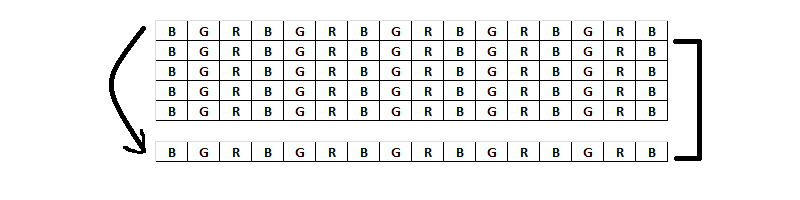
\includegraphics[scale=0.7]{imagenes/mover1.png}
\end{center}

\item El otro propuesto fue, levanar esos 5 registros pero en lugar de mover 1 registro hacia abajo, aprovechar la cache del procesador moviendonos hacia
la derecha ya que cuando copiamos de memoria un registro de 16 bytes traemos con el mucha mas informaci\'on que queda en cache con lo cual al movernos hacia
de esta manera estamos aprovechando los HIT de la cache en lugar de un MISS por cada iteraci\'on del ciclo. A continuaci\'on una imagen de lo propuesto.\newline
\begin{center}
 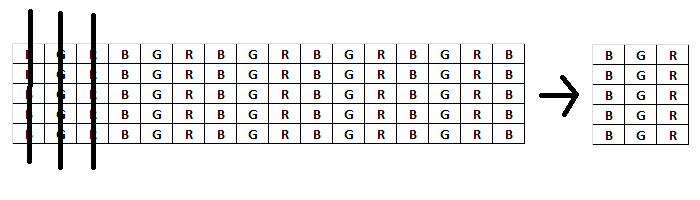
\includegraphics[scale=0.7]{imagenes/mover2.png}
\end{center}
Finalmente se opto por la segunda opci\'on por cuestiones de performance. El resto de las cuestiones estructurales como ciclos y operaciones son muy
similares al C.
\end{itemize}


\subsubsection{Resultados}
Comparando ambas implementaciones, notamos que estructuralmente no cambian mucho. En ambas tenemos la misma idea de ir recorriendo las bandas por un lado e ir haciendo la cuenta para el nuevo p\'ixel por otro. De todas formas, lo que se destaca es que en ASM tenemos menos accesos a memoria, ya que procesamos de a 5 p\'ixels, mientras que en C lo hacemos de a uno.\\
Adem\'as se puede apreciar que el ensamblado del compilador de C, al no usar SIMD se producen m\'as comparaciones que el ASM para terminar de recorrer la im\'agen.
En cuanto a la performance confirmamos lo que hab\'iamos supuesto, el ASM result\'o ser m\'as r\'apido que el C.\\

\begin{center}
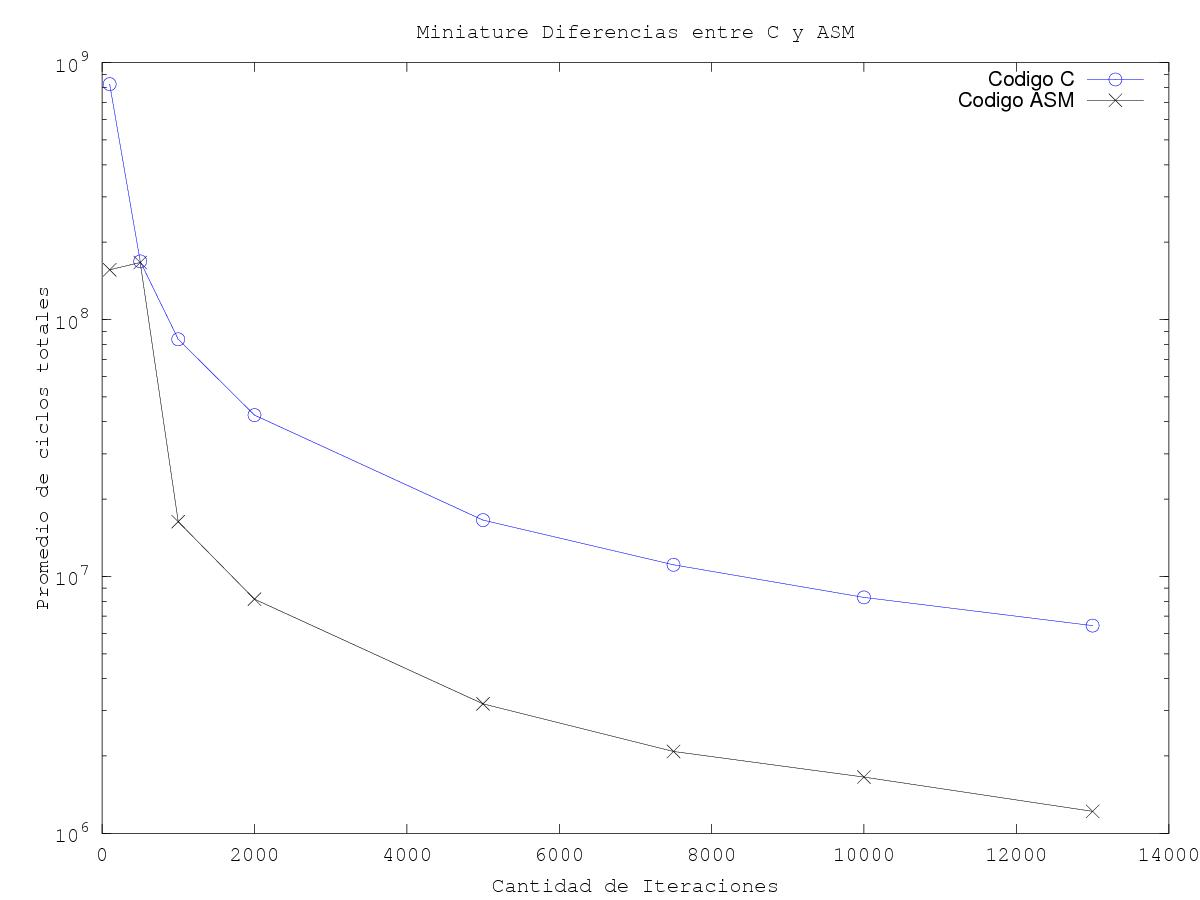
\includegraphics[width=16cm]{imagenes/medicionMiniature.jpg}  
\end{center}

Como podemos ver en el gr\'afico, lo que tarda la ejecuci\'on en promedio, el C se mantiene a la misma distancia del ASM a medida que aumentan las iteraciones, siempre tardando m\'as tiempo.\\

Experimentamos con varios tamaños de im\'agenes y pudimos ver que la diferencia en velocidad no cambia mucho. El C sigue tardando m\'as que el ASM, y con im\'agenes mas grandes hasta puede tardar m\'as que lo que vimos en el gr\'afico anterior.\\
Consideramos que a la hora de hacer este tipo de filtros, lo m\'as prioritario para optimizar es es evitar los accesos a memoria lo m\'as posible, ya que como sabemos es una de las cosas m\'as costosas que hay.\\





\subsection{Decodificaci\'on Esteganogr\'afica}

El filtro Decode, obtiene un mensaje a partir de los bytes de la entrada, proces\'andolos primero y luego qued\'andose con los bits relevantes para la 
decodificaci\'on.

\subsubsection{Implementación en C}
En un ciclo principal, se recorren los bytes de la fuente, hasta terminar de recorrer la imagen o alcanzar el tamaño recibido por par\'ametro. Dentro de 
este ciclo hay otro, que recorre de a 4 bytes. Los obtiene primero el c\'odigo de la operación a aplicar, luego los bits que ser\'an procesados y luego 
se realiza el algoritmo correspondiente. En cada iteraci\'on del ciclo interior, en una variable que contiene el byte decodificado, inserta los bits 
procesados en la posici\'on que les corresponde. Al terminar con el cuarto byte, pega ese valor en la salida y avanza los punteros y variables para 
continuar con el siguiente grupo de bytes.

\subsubsection{Implementación en Assembler}
El ciclo del algoritmo obtiene en primer lugar 16 bytes de la fuente. Luego, con una m\'ascara obtengo los bits 2 y 3 de cada byte en un registro. Luego 
con otras m\'ascaras, se obtienen los bytes a los que se les debe sumar 1 en un registro y a los que se debe restar 1 en otro. El pr\'oximo paso, niega 
los bits de los bytes cuyo c\'odigo de opraci\'on es 3. A ese resultado, se le suma 1 al registro usando la m\'ascara obtenida anteriormente, y lo mismo 
se hace para restar 1 usando la otra m\'ascara. Despu\'es de eso, se borran todos los bits que no interesan, dejando solo los bits 0 y 1 de cada byte.\newline
Para juntarlos y armar los bytes decodificados, en diferentes registros, se dejan solo los pares de bits que van en las posiciones 0 y 1, 2 y 3, 4 y 5 , 
6 y 7. Luego, con pshufb y las m\'ascaras correspondientes, llevo esos bits manteniendo sus posiciones, pero a los primeros 3 bytes del registro. Y 
finalmente con la instrucci\'on POR se guardan en un solo registro todos los bits en su posici\'on correspondiente. Finalmente se guarda ese registro en 
la posición del output. Como solo los primeros 3 bytes eran reelevantes para el output, el puntero se avanza solo 3 lugares. En la fuente en cambio, 
aumento 12 lugares la posici\'on. Esto se hace as\'i porque cada pixel ocupa 3 bytes, y para formar un byte de la salida se necesitan 4 bytes. Avanzar de
 a 12 la fuente y de a 3 el destino entonces, es conveniente para avanzar de forma m\'as ordenada y segura.

\subsubsection{Resultados}
La diferencia principal entre el c\'odigo escrito en lenguaje C y el c\'odigo ASM, es la cantidad de accesos a memoria realizados en cada iteraci\'on. Otra diferencia puede verse en la cantidad de bytes que puden ser procesados simultaneamente durante el mismo ciclo. Mientras que en C leemos y procesamos un byte por vez, el c\'odigo ASM nos permite acceder y procesar 16 bytes en simultaneos. De todas maneras, en este caso trabajamos con 12 bytes que es un numero mas \'util ya que es múltiplo de 3 (cantidad de bytes pos pixel)  y de 4 (cantidad de bytes por cada caracter).
\newline
Pudiendo levantar de a 16 bytes en memoria, podr\'ia esperarse que el c\'odigo asm demorase una diesiseiava parte de la cantidad de ciclos que demora el c\'odigo en C. Pero debemos tener en cuenta que en nuestro caso estamos aprovechando solo 12 de los 16 bytes que leemos en cada iteraci\'on por lo tanto es más acertado evaluar como si solo leyeramos 12 bytes. Adem\'as, hay que tener en cuenta que las instrucciones SSE pueden necesitar más ciclos que las operaciones comunes que usamos en el C, eso disminuye un poco la performance en la comparación. Viendo el promedio de ciclos necesitados por cada c\'odigo en promedio, estamos en la mayor\'ia de los casos en cifras cercanas a 10.35, por lo tanto, concluimos que para la mayoría de los casos, esa es la relaci\'on de performance entre los códigos.
\newline

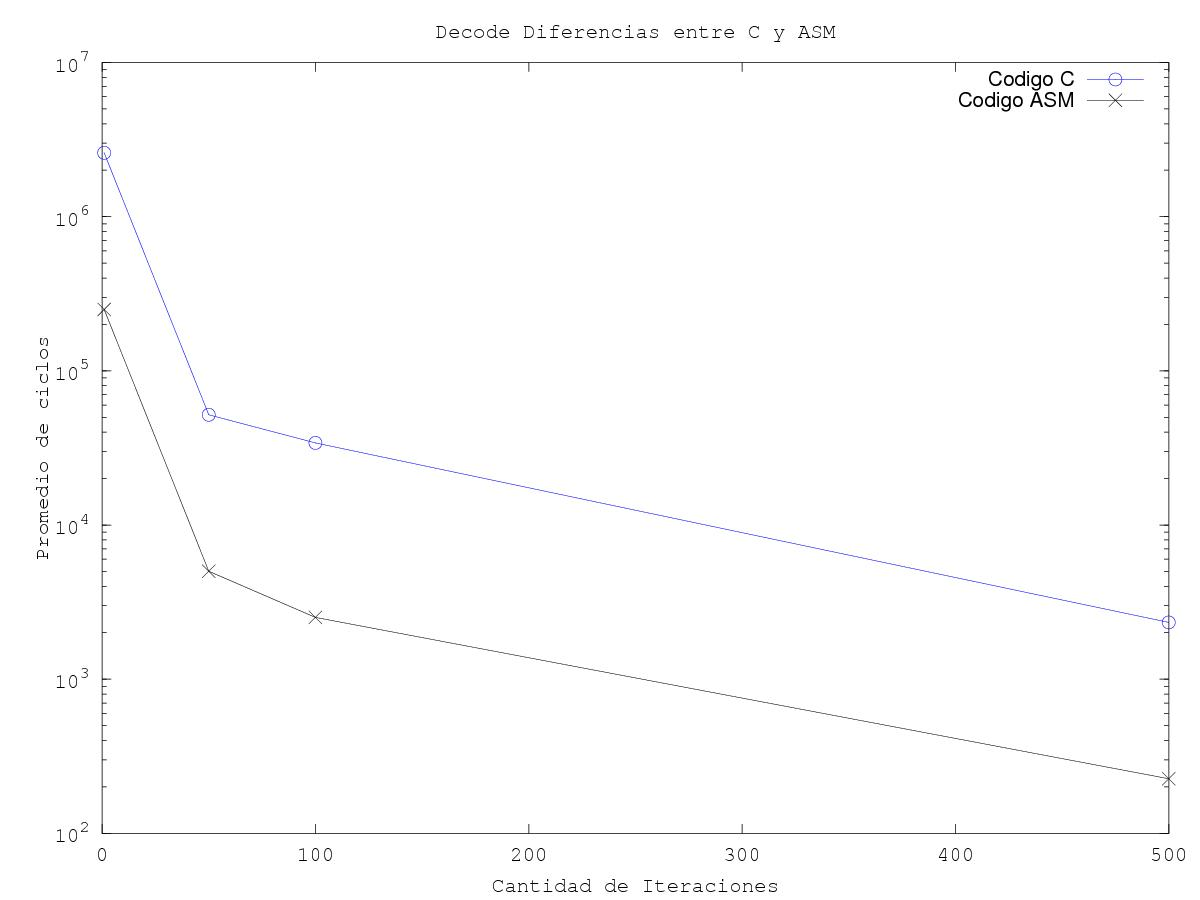
\includegraphics[scale=0.7]{imagenes/octave1.jpg}

Probando con im\'agenes de distintos tamaños, una de 1920 X 1080 p\'ixeles y otra de 640 x 480 p\'ixeles, sucedi\'o en ambos casos que hubo un aumento en la diferencia entre los c\'odigos, pero se mantuvo, para las dos im\'agenes y, para distinta cantidad de iteraciones, un promedio de aproximadamente, por lo que no presentan grandes cambios con la imagen original. 

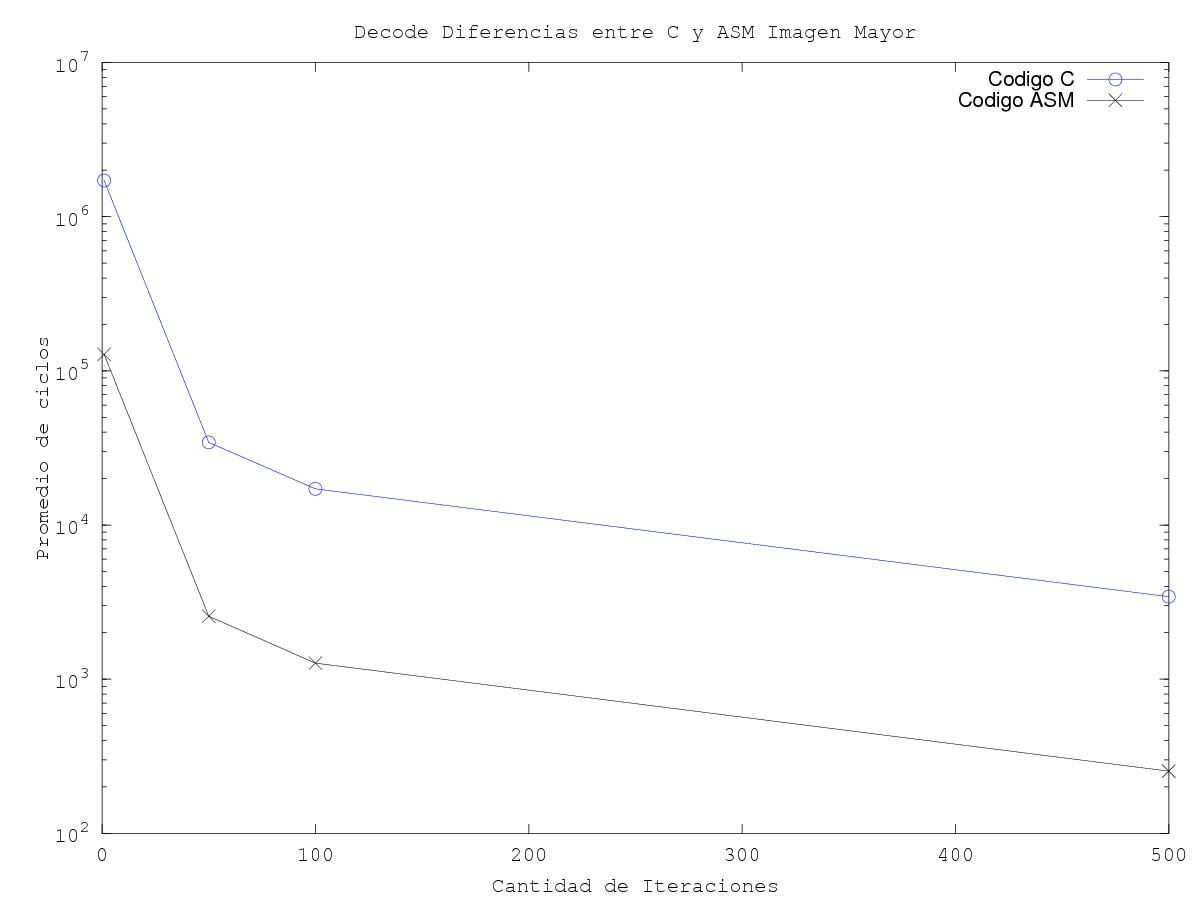
\includegraphics[scale=0.7]{imagenes/DecodeMayor.jpg}

%falta el grafico de imagen de menor tamaño.

Para desarrollar el codigo con la tecnica de pipelining, lo primero que modificamos fue el uso de los regitros. Intentando de hacer cada seccion del codigo con registros distintos para disminuir la dependencia entre las instrucciones. Una vez logrado esto, el aumento de performance fue muy significativo. Realizar una iteracion del codigo nos costaba antes aproximadamente 250200 ciclos del clock y, con la nueva tecnica logramos reducir el tiemo a aproximadamente 115362 ciclos.
\newline
Luego intentamos intercalar algunas instrucciones para reducir aun mas la cantidad de ciclos necesarios, pero no se lograron cambios apreciables.
\newline
\newline
En cuestion de performance, se puede apreciar en el siguiente grafico, que se ha logrado un salto en la cantidad de ciclos bastante importante. En el codigo C, en coomparacion con el ASM sin pipelining, demoraba aproximadamente 10.36 veces mas. La diferencia se lograba gracias a la posibilidad de leer de la memoria de a 16 bytes por cada acceso en lugar del unico que podiamos leer en C. Luego, una vez utilizada la tecnica de pipelining, podemos apreciar que la diferencia es aun mayor, logrando que en C se demore aproximadamente 22.48 veces más que utilizando pipelining en ASM. Y el ASM sin pipelining demora aproximadamente 2.17 veces mas que el que si utiliza esta tecnica.
\newline

%falta el grafico de pipelining




%%%%%%%%%%%%%%%%%%%%%%%%%%%%%%%%%%%%%%%%%%%%%%%%%%%%%%%%%%%%%%%%%%%%%%%%%%%%%%%
%% Conclusión                                                                %%
%%%%%%%%%%%%%%%%%%%%%%%%%%%%%%%%%%%%%%%%%%%%%%%%%%%%%%%%%%%%%%%%%%%%%%%%%%%%%%%


\section{Conclusión}

Las instrucciones SIMD (Single Instruction Multiple Data) proveen al programador de una herramienta más efectiva para realizar el mismo conjunto de operaciones a una gran cantidad de datos.

La aplicación del filtros a imágenes era un ejemplo perfecto para probar su eficiencia.

Analizando los resultados de las implementaciones de los 6 filtros, podemos notar:

\begin{itemize}
\item Las operaciones básicas (padd, psub, pmul, pdiv, shifts, etc.) SIMD tienen un costo similar a sus correspondientes operaciones unitarias, pero generalmente requieren algún tipo de preproceso para poder trabajar con los 16 bytes (pack, unpack, shifts) en una sola iteración, por lo tanto, aunque más eficientes, no lo son en una relación directamente proporcional.
\item En el caso que sí hay una relación directamente proporcional es en el acceso a memoria (como se comprobó en el filtro recortar).
\item Además, el acceso a memoria es, por lejos, la operación más costosa de las que implementamos en cada filtro.
\item Por consecuencia directa del ítem anterior, las llamadas a otras funciones (que a su vez, probablemente contengan variable locales) dentro de una iteración provocan estragos en la efectividad de las implementaciones en C.
\item Para poder aprovechar las instrucciones SIMD es un prerequisito que los datos estén contiguos en memoria. Como descubrimos con el filtro Rotar, los datos dispersos nos obligan a hacer múltiples lecturas a memoria y perder tiempo reordenándolos dentro de los registros antes de poder procesarlos.
\end{itemize}

Concluimos que, definitivamente, las instrucciones SIMD, cuando pueden aprovecharse, demuestran una gran eficiencia. Sin embargo, hay que tener algunas consideraciones:

Aunque las imágenes, video y sonido son los primeros candidatos a ser optimizados por paralelización, no todos los procesos pueden ser efectivos y se requiere un análisis profundo de los datos para ver si vale el esfuerzo.

Además, aunque se pueda lograr una gran optimización, no siempre es lo más importante. Ninguno de los filtros implementados demoró más de 1 segundo en ejecutarse completamente. La optimización seguramente es indispensable en transmisiones de video en vivo, pero baja en importancia si tuviese que ser aplicado una sola vez en una aplicación tipo MS Paint.

Las desventajas que podrían opacar a la optimización son:

El código no es portable, únicamente funciona en procesadores que implementan el set de instrucciones AMD64, requiriendo reescrituras para otras plataformas. Sin embargo el código C debería funcionar perfectamente en IA-32, ARM y cualquier otro procesador que tenga un compilador de lenguaje C.

El código es mucho más largo y difícil de entender (por lo tanto mayor posibilidad de tener bugs) que en un lenguaje de más alto nivel como C. Y en pos de la optimización, se llegan a eliminar funciones (poniéndolas inline), lo que genera código repetido, largo y confuso.




\end{document}